\documentclass[12pt,a4paper,notitlepage]{article}
\linespread{2.0}

\usepackage[T1]{fontenc}
\usepackage[utf8]{inputenc}
\usepackage{hyperref}
\usepackage{mathtools}
\usepackage{graphicx}

\begin{document}

\title{Technical Report on Convolutional Neural Networks}
\author{Sebastien Champoux
\\ 40133449
\\ Concordia University
\\ ENGR 411 Technical Report
}
\maketitle

\begin{abstract}
I'm baby semiotics salvia literally +1 af coloring book woke banh mi gentrify organic wolf 8-bit tote bag chartreuse chicharrones. Helvetica cardigan next level art party kickstarter, vexillologist banh mi master cleanse actually street art tumeric poke whatever.
\end{abstract}
\clearpage

\tableofcontents
\clearpage

\listoffigures
\clearpage

\section{Introduction}
[Talk about the fact that we are talking about image classification specifically.]

\section{Multilayer perceptron}\label{multilayer-perceptron}
Convolutional neural networks are a variation of multilayer perceptrons, a common class of neural networks. Therefore, it makes sense to start there.

\subsection{Structure}
A classical concrete application of a neural network is the identification of handwritten digits. This application is commonly used as an example thanks to the existence of the MNIST Database (\textit{Modified National Institute of Standards and Technology database}), a database of 70,000 labelled pictures of handwritten digits freely available for machine learning \cite{lecun_mnist_1998}. To simplify the presentation of multilayer perceptrons below, this application will be used to illustrate how the different components of a neural network can work together to achieve this application.

A multilayer perceptron is a class of neural network. As the name implies, it is made up of "neurons" that are connected together. A neuron is simply a real number in the range [0,1] that represents an activation; 0.0 meaning the neuron is not activated and 1.0 meaning the neuron is fully activated. The neurons are arranged in multiple layers, at least three: an input layer, an output layer, and at least one "hidden" layer, each one serving a different role.

Each neuron in the input layer represents a part of the total input provided to the perceptron. For the digits example, the input is a black and white image of a handwritten digit, of format 28*28 pixels. Therefore, the input layer would constitute of 784 neurons, each corresponding to a pixel of the image, and their respective activation being the brightness value of their respective pixel (0.0 being black, 1.0 being white, and shades of grey in-between) \cite{sanderson_but_2017}.

The output layer represents the output of the neural network. As the perceptron performs recognition and classification, each neuron in the output layer is one of the possible "choices" of what could be represented in the image. For the digits example, the output layer would contain ten neurons, one for each digit. The intended output of the neural network is for all but one of the output neurons to have a low activation, and one neuron having a very high activation, the latter being the network's best guess of what digit is represented in the image.

The hidden layers, in-between the input and output layers, serve to improve the performance of the neural network. These layers enable the network to recognize patterns within the image, therefore facilitating the recognition of complex forms. For instance, the digit "8" is made up of two small loops one over the other. In theory, the middle layers could attempt to recognize these shapes in the image to make a decision whether the digit represented is an eight. In practice, neural networks create their own patterns during the training process, which are often very abstract and a far cry of what a human would consider logical \cite{sanderson_gradient_2017}.

In a standard multilayer perceptron, every neuron from a layer is connected to every neuron from the previous layer. The activation of a neuron impacts the activation of every neuron connected to it ; in other words, with the exception of the input layer, neurons are functions of the activation of the neurons that preceed them. The connection in-between two layers can be weighted, to increase or decrease how much the activation of a neuron impacts the connection of another neuron.

\begin{figure}[htbp]
	\centering
		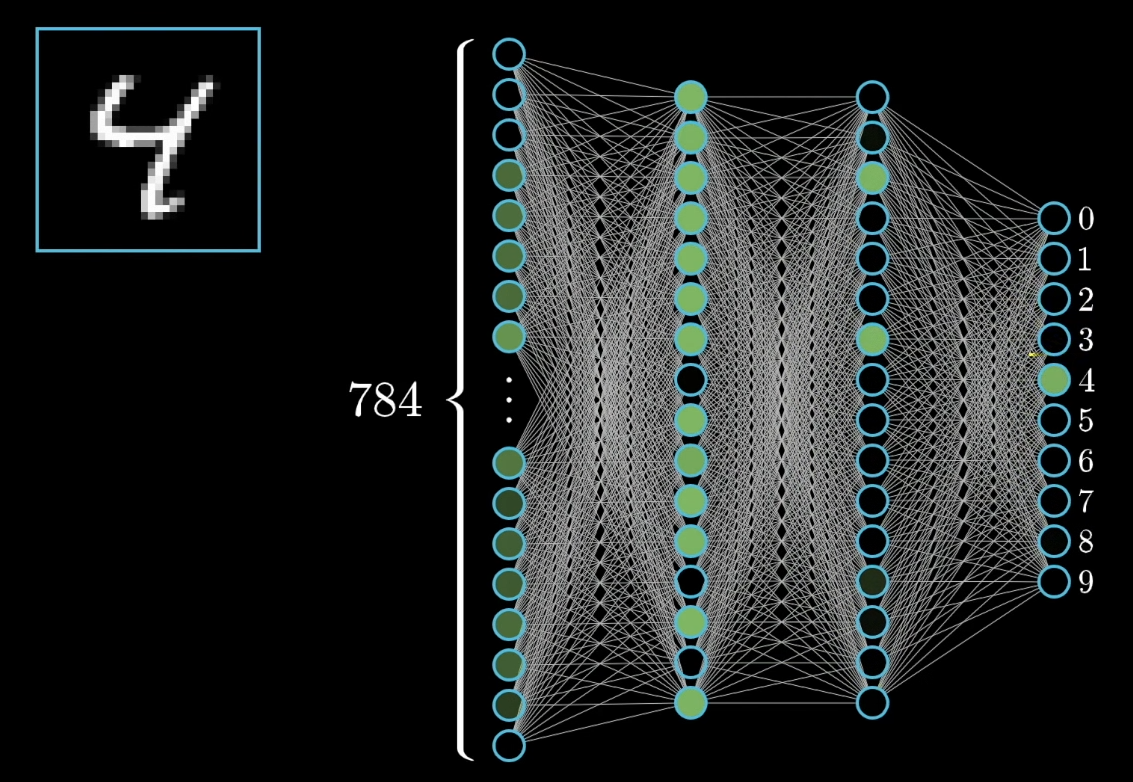
\includegraphics[width=0.60\textwidth]{images/perceptron-visualisation.png}
	\caption{Visualisation of a multilayer perceptron \cite{sanderson_gradient_2017}}
	\label{fig:perceptron-visualisation}
\end{figure}

A bias can also be introduced into the equation. The addition of a bias can help improve the results by requiring a very high, or very low, activation in parts of the input layer before activating some specific neurons in the following layers \cite{sanderson_but_2017}.

All of these elements can be summarized into a vector-matrix multiplication. Below is the equation to compute the activation of the neurons in hidden layer 1, based on the activation of neurons from the input layer (layer 0). \(a_i^{(0)}\) represents the activation of neuron \(i\) from layer 0, \(w_{i,j}\) the weight of the connection between neuron \(i\) from the input layer and neuron \(j\) in layer 1, and \(b_i\) the bias applied to the weighted sum of the incoming connections from all of layer 0 to neuron \(i\) in layer 1. This output vector is processed through a function, usually the sigmoid function, to squish the results into the range \([0,1]\). This output neuron represents the activation of every neuron in layer 1. This process can then be repeated for the subsequent layers, using the activation vector of layer 1 as input \cite{sanderson_but_2017}.

\begin{displaymath}
	\sigma
	\left(
	\begin{bmatrix}
		w_{0,0} & w_{0,1} & \cdots & w_{0,n}\\
		w_{1,0} & w_{1,1} & \cdots & w_{1,n}\\
		\vdots & \vdots & \ddots & \vdots\\
		w_{m,0} & w_{m,1} & \cdots & w_{m,n}
	\end{bmatrix}
	\begin{bmatrix}
		a_{0}^{(0)}\\
		a_{1}^{(0)}\\
		\vdots\\
		a_{n}^{(0)}
	\end{bmatrix}
	+
	\begin{bmatrix}
		b_{0}\\
		b_{1}\\
		\vdots\\
		b_{n}
	\end{bmatrix}
	\right)
	=
	\begin{bmatrix}
		a_{0}^{(1)}\\
		a_{1}^{(1)}\\
		\vdots\\
		a_{n}^{(1)}
	\end{bmatrix}
\end{displaymath}

As demonstrated above, a neural network boils down to fairly simple, albeit large, linear algebraic functions. For this reason, neural networks are often computed by graphical processing units (GPU) instead of regular CPUs, as the formers are optimized for processing vector-matrices computations \cite{salter_cart_2021}.

\subsection{Deep learning, gradient descent and backpropagation}
\subsubsection{Description of the process}
Once the structure of the neural network has been laid down, it must be tuned so that it can recognize and classify accurately what is presented to it. This tuning process consists of adjusting the hundreds of weights and biases in-between neurons, in order for a given input to trigger the appropriate activations in the output layer with an acceptable rate of accuracy. It goes without saying that this is too tedious and intricate to be performed by humans. Therefore, the neural network "trains itself" with the help of two algorithms, gradient descent and backpropagation. \cite{ibm_cloud_education_what_2020}.

To train a neural network, it is necessary to have a training set on-hand. A training set is a set of contents (images, videos, audio clips or some other medium), each item of which is labelled with the expected classification. As discussed earlier, the MNIST database is a good example of a training set: it is a set of 70,000 images of hand-drawn digits, each image appropriately labelled with the represented digit \cite{lecun_mnist_1998}. Another example is the database created by Google's ReCAPTCHA service. This service helps to protect websites from bots by asking web users to identify objects within images. By doing so, human users of ReCAPTCHA are also, unknowingly, contributing to the elaboration of training sets for AI training \cite{maruzani_are_2021}.

To begin the training process, the different weights and biases of the neural network are initialized with random values. Then, the training set is processed by the neural network. Unsurprisingly, the results will be very poor at this stage. The network computes the accuracy (or lack thereof) of its results with a cost function. This function receives, as input, the different weights and biases in the neural network, and returns a real number, the cost of the network's errors. This cost is computed by averaging the error cost of each element in the training set.

Below is the cost function of the neural network for one element of the training set. It is the sum of the squared difference between the activation of each neuron in the output layer (\(a_{j}^{(L)}\)) and their expected activation (\(y_{j}^{(L)}\)). These error costs are averaged to get an error costs for the neural network over the training set.
\begin{displaymath}
	C_{0} = \sum_{j=0}^{n_{L} - 1} (a_{j}^{(L)} - y_{j})^{2}
\end{displaymath}
This cost function expresses how accurate the results given by the neural network are. The higher the error cost, the greater the difference between the expected and computed results and thus, the less accurate the network. The objective is to adjust the weights and biases in the neural network to decrease this error cost as close as possible to 0 for the training set.

To reduce this cost function, gradient descent will be used. Gradient descent is an optimization algorithm to find a local minimum of a function. It consists of computing the gradient of a function (noted \(\nabla C\) - a vector in the direction of the steepest increase), adjusting the function by a factor of the negative of this vector (\(-\nabla C\)), and repeating these steps until a local minimum is reached \cite{sanderson_gradient_2017}.

The algorithm to efficiently compute the gradient of a neural network is backpropagation. This algorithm computes the adjustments that should be made to every weight and bias in the neural network in order to minimize the error cost. For each element in the training set, the algorithm starts from the output layer, and compares the activation of the output layer's neurons to the expected result. Then, it computes by how much each weight and bias that connect the output layer to its previous layer should be adjusted in order to minimize the error cost (in other words, decrease the difference between the output neurons' actual and expected activation). Connections (weights) that improve the accuracy of the results should be strengthened, and inversely, connections that worsens the results should see their weight diminished. Furthermore, these adjustments should be proportional to how much each connection impacts the error cost. This procedure is repeated recursively for each layer in the neural network. Finally, the adjustments computed for each example in the training set are averaged to get an adjustment vector for the entire training set. This algorithm is repeated multiple times until an acceptable accuracy is reached \cite{sanderson_gradient_2017}.

\subsubsection{Calculus of deep learning}
The process above is achieved through the use of derivatives and the chain rule of calculus.

The equation below is the weighted sum of the activation of the neurons of the previous layer, plus a bias. In other words, it is the activation of a neuron that has not yet been processed through the sigmoid function. Note that this weighted sum is represented as \(z_j^{(L)}\) to differentiate it from the activation of a neuron (represented as \(a_j^{(L)}\) in the second equation below). This equation is presented here separately from the activation function because it will be used to compute the cost function's gradient.
\begin{displaymath}
	z_j^{(L)} = w_{j0}^{(L)}a_0^{(L-1)} + w_{j1}^{(L)}a_1^{(L-1)} + \cdots + w_{jk}^{(L)}a_k^{(L-1)} + b_j^{(L)}
\end{displaymath}

Thus, the activation for a neuron in the neural network can be represented as:
\begin{displaymath}
	a_j^{(L)} = \sigma\left(z_j^{(L)}\right)
\end{displaymath}

The derivative of the cost function over the derivative of a specific weight is necessary for this computation. It is represented in the equation below. Not all connections in the network have an equal impact on the error cost ; this equation tells us how much a specific weight or bias in the neural network impacts the error cost.
\begin{displaymath}
	\frac{\delta C_0}{\delta w_{jk}^{(L)}} = a^{(L-1)} \sigma\prime(x^{(L)})((a^{(L)})^2)\prime
\end{displaymath}

Below: derivative of cost function in relation to a specific activation. Tells how sensitive cost is to a specific activation in the previous layer (L-1). Neuron influences cost through multiple different "paths" which is why we sum those influences together.
\begin{displaymath}
	\frac{\delta C_0}{\delta a_{k}^{(L-1)}} = 
	\sum_{j=0}^{n_{L-1}}
	\frac{\delta z_j^{(L)}}{\delta a_{k}^{(L-1)}}
	\frac{\delta a_j^{(L)}}{\delta z_j^{(L)}}
	\frac{\delta C_0}{\delta a_j^{(L)}}
\end{displaymath}

Therefore, by using the chain rule, it is possible to compute the derivative of the cost function in relation to a specific weight. This equation tells us how much an adjustment to this weight will impact the error cost.
\begin{displaymath}
	\frac{\delta C_0}{\delta w_{jk}^{(L)}} = 
	\frac{\delta z_j^{(L)}}{\delta w_{jk}^{(L)}}
	\frac{\delta a_j^{(L)}}{\delta z_j^{(L)}}
	\frac{\delta C_0}{\delta a_j^{(L)}}
\end{displaymath}

The result is the gradient descent vector. Each component of this vector represents the adjustments that should be made to the different weights and biases in the neural network to minimize the cost function.
\begin{displaymath}
	-\nabla C =
	-1 \begin{bmatrix}
		\frac{\delta C_0}{\delta w_{0,0}^{(1)}}\\
		\frac{\delta C_0}{\delta w_{0,1}^{(1)}}\\
		\vdots\\
		\frac{\delta C_0}{\delta w_{j,k}^{(1)}}\\
		\frac{\delta C_0}{\delta b_{0}^{(1)}}\\
		\vdots\\
		\frac{\delta C_0}{\delta b_{k}^{(1)}}\\
	\end{bmatrix}
\end{displaymath}

It should be noted that computing the error cost and gradient descent of a neural network over a training set of tens of thousands of examples is computationally expensive. For this reason, a more performant technique, stochastic gradient descent, is commonly used. The algorithm is the same, but instead of computing the entire training set, the training set is subdivided into multiple smaller random subsets of training examples. Then, the gradient descent vector is computed for every subset of the training set, and these vectors are applied iteratively to gradually improve the results of the network \cite{sanderson_gradient_2017}.

[FORMULA?]

\section{Convolutional neural networks}

\subsection{Image convolutions}
Image convolutions is a technique of image processing to create different renditions of images, such as blurring, sharpening, highlighting edges, etc. It consists of applying a kernel, i.e., a small matrix, over the image, by image convolutions. An image convolution consists of computing the weighted average of the values of each group of pixel of the same size as the kernel, according to the pixel weights defined in the kernel \cite{sanderson_convolutions_2020}.

\begin{displaymath}
	\begin{bmatrix}
		1/9 & 1/9 & 1/9 \\
		1/9 & 1/9 & 1/9 \\
		1/9 & 1/9 & 1/9
	\end{bmatrix}
\end{displaymath}

\begin{figure}[htbp]
	\centering
		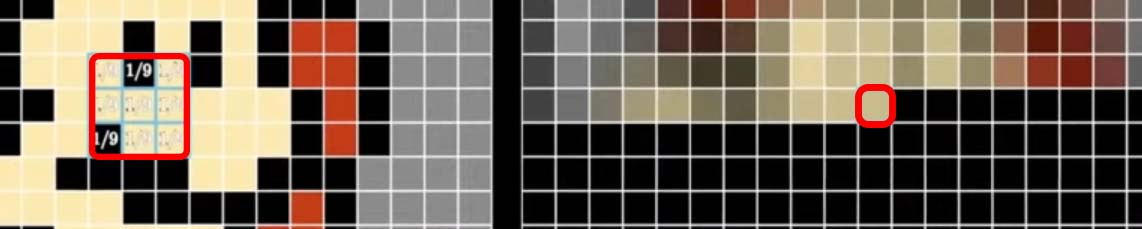
\includegraphics[width=1.00\textwidth]{images/box-blur.jpg}
	\caption{A group of beige and black pixels are averaged to a grey-beige by the box blur kernel \cite{sanderson_convolutions_2020}.}
	\label{fig:box-blur}
\end{figure}

As a simple example, the kernel above would create a box blur effect. For each group of 9 pixels in the original image, the corresponding center pixel in the blurred image would be equal to an average of the 9 pixels, all with equal weights.

Another example of a possible simple kernel is \(\begin{bsmallmatrix}-1 & -1 & -1 \\ 1 & 1 & 1 \\ 0 & 0 & 0\end{bsmallmatrix}\). This kernel would highlight top edges of objects in an image \cite{deep_lizard_convolutional_2017}.

\begin{figure}[htbp]
	\centering
		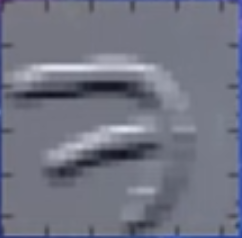
\includegraphics{images/edge-highlighting-kernel.png}
	\caption{The rudimentary kernel above highlights the top edges of this handdrawn seven \cite{deep_lizard_convolutional_2017}.}
	\label{fig:edge-highlighting-kernel}
\end{figure}

\begin{figure}[htbp]
	\centering
		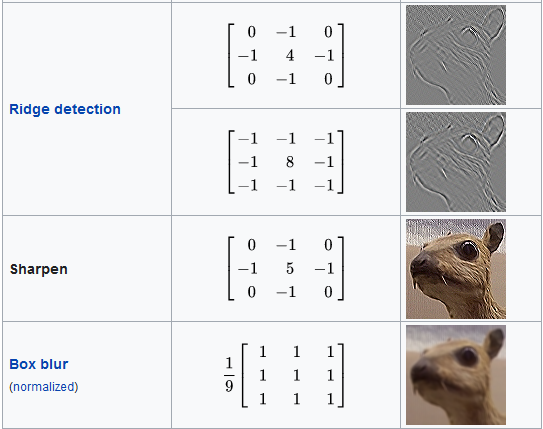
\includegraphics[width=0.8\textwidth]{images/image-convolutions-examples.png}
	\caption{Other examples of kernels and their application on a sample image \cite{wikipedia_collaborators_kernel_2022}}
	\label{fig:image-convolutions-examples}
\end{figure}


\subsection{Using image convolutions in a neural network}
As the name may suggest, a convolutional neural network is a multilayer perceptron, as seen in section \ref{multilayer-perceptron}, that uses image convolutions to extract information from images in order to facilitate their classification \cite{deep_lizard_convolutional_2017}.

\subsection{Concrete applications of CNNs}

\section{Favorable characteristics of CNNs for image recognition}

Keeps spatial data instead of flattening the image \cite{saha_comprehensive_2018}
Not fully connected = lighter and more efficient than a regular multilayer perceptron
Use of different filters = enables extraction of many kinds of data
More possibilities (for ex not just classification. Identification also possible)

\section{Conclusion}

\clearpage
\begin{flushleft}
\bibliographystyle{plain}
\bibliography{references}
\end{flushleft}

\end{document}